\subsection{Task overheads}
Having discovered that a significant portion of the time spent running small tasks is in deserialization, we further measured the time it took individual components of deserialization to complete. Figure \ref{fig:deserialization} summarizes the workflow of task deserialization on the executor.An array of bytes called serializedTask is deserialized into a tuple of taskFiles, taskJars, and taskBytes, the first two of which are passed into a method called updateDependencies, while the latter is further deserialized into a Task object. The Task object contains information such as the function to run, the RDD (Resilient Distributed Dataset, Spark's abstraction for distributed objects) to use, and the partition of the RDD to operate on.


\begin{figure}[t!]
  \begin{center}
    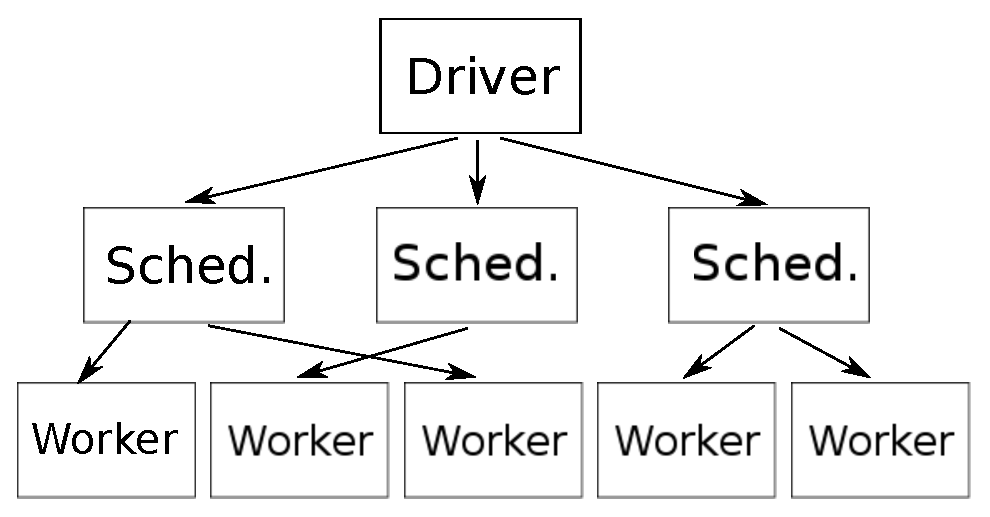
\includegraphics[scale=0.45]{scheduler_architecture.eps}
  \end{center}
  \caption{Proposed scheduler architecture. Schedulers are oportunistically spawned by the driver. These schedulers receive tasks from the Driver and schedule them to Worker nodes.}
  \label{fig:schedarch}
\end{figure}

What we found is that in order to reduce the amount of duplicate data transferred, Spark 1.1.0 wraps the function and the RDD into a broadcast variable. This way, each executor will only fetch the function and the RDD of a batch once. The first task that uses the information will pull it from the driver, and cache the result within the executor for later tasks. In the Spark Streaming context however, this means for every stage, some task on every executor requires a round trip to the driver to fetch the broadcast variable, increasing the latency. As the batch interval shrinks, new RDDs are created more often, but the functions to operate on them do not change. The executor should be able to cache them for a longer period of time than only for the current stage. We have reverted the implementation to not use the broadcast variable, and have already seen latency improvements when the number of executors is relatively small. We plan to further optimize this part by caching functions across stages.

Another interesting discovery regarding the deserialization time is that in updateDependencies(), the current implementation creates a new Hadoop configuration object regardless of whether new dependencies are introduced. However, this objection creation is very costly in CPU cycles. We have changed the object to be lazily instantiated, and are already seeing an order of magnitude improvement in the execution time of that function.


\subsection{Scheduling Scalability}


To enable a higher scheduling rate of tasks by Spark Streaming we propose 1) scheduling all tasks per worker in bulk and 2) physically decoupling the scheduling (Scheduler) of tasks from their generation (Driver).
First, at each scheduling stage, instead of sending multiple tasks for each node separately, we coalesce them into the same message. This reduces the serialization and networking overheads that result from sending many small messages.
Secondly, as the task generation rate surpasses the scheduling rate, the driver elastically spawns schedulers in remote physical nodes. Thereafter, tasks are forwarded, according to some policy, to these newly spawned schedulers for scheduling (see Figure \ref{fig:schedarch}). 

We have implemented this decentralized architecture in Spark Streaming. Due to the instability of connections between the schedulers, the driver and the workers -- connections are dropped after running the system for a few minutes -- we are currently not able to evaluate the performance benefits of this technique. We plan to fix this engineering problem and report on further results.


\subsection{Network Overhead}
We plan to look into the proposed solutions in this area next.
